\begin{figure}
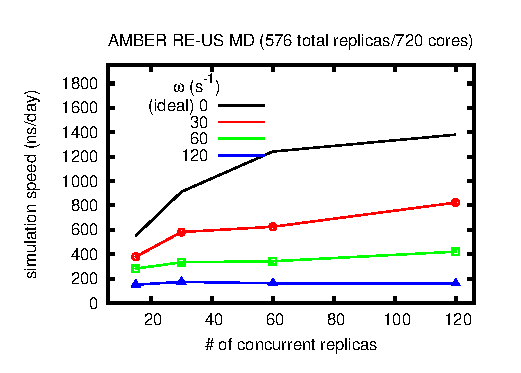
\includegraphics[width=3in]{amber_data/amber_mm.eps}
\caption{
  Scaling results for ASyncRE/BigJob with the AMBER MD engine employing a
  scalable molecular mechanics force field. Each run consisted of 720 cores
  divided amongst differing numbers of replicas (the pool of potential 
  replicas was fixed at 576). Ideal performance (black line) would be obtained
  if there is no overhead in launching or coordinating simulations. Increasing
  the frequency with which replicas are ``launched'' results in diminished
  performance, although the penalty for doing so appears to be fairly uniform
  at higher frequncies (blue line).
  \label{fig:amber_mm}  
}
\end{figure}

Standard REMD simulations employing molecular mechanics (MM) force fields offer 
parallel scaling in both the number of replicas and the number of processors 
allocated to each replica. An optimal scheme should balance the efficiency 
gains of both types of scaling in order to produce the most simulation time in 
real time. In order to assess the efficiency of ASyncRE/BigJob in combination 
with the AMBER MD engine, a fixed size pilot job of 720 cores was allocated 
(AMBER system 1 under Experimental Configuration) with various numbers of cores
allotted to each simulation. In this scheme, the number of simulations being 
coordinated in REMD varies, as well as the simulation rate (in ns/day) attained
by each replica. In order to probe the efficiency with which ASyncRE/BigJob 
coordinates simulations, the length of each simulation cycle (alternatively the 
frequency with which simulations are coordinated) was fixed in real time by 
varying the simulation time per cycle (Figure \ref{fig:amber_mm}). Ideal
performance would be obtained if there is no overhead in coordinating 
simulations. However, some cost must be incurred both in starting, stopping,
and restarting simulation cycles as well as in coordinating exchanges amongst 
stopped replicas, and the cost of this overhead is expected to increase as the 
frequency with which it is incurred increases. As seen in Figure 
\ref{fig:amber_mm}, this cost does indeed result in diminished output (as 
measured in ns/day) as the coordination frequency increases. However, for a
fixed coordination interval, the overhead appears to level out as a function
of the number of simulations being coordinated. This means that, at present, 
one can generally increase the number of replicas being simulated with only a
minor hit to performance.

\brnote{Move this to the discussion?}
Although in general one wants to produce as much simulation time as possible, 
it is worthwhile to note that not all simulation time is equal, in the sense 
that multiple short simulations do not usually contain as much statistical 
information as a single short simulation. In fact, the basic aim of REMD is to
increase the statistical power of multiple simulations by facilitating the
exchange of information between them in a concerted fashion. This should be
kept in mind when analyzing performance graphs, as one might be tempted to run
as many small simulations as possible in an attempt maximize simulation speed.
For real applications and performance optimizations, other more physically and
statistically relevant metrics must be employed, but these are beyond the
scope of the present work.

\begin{figure}
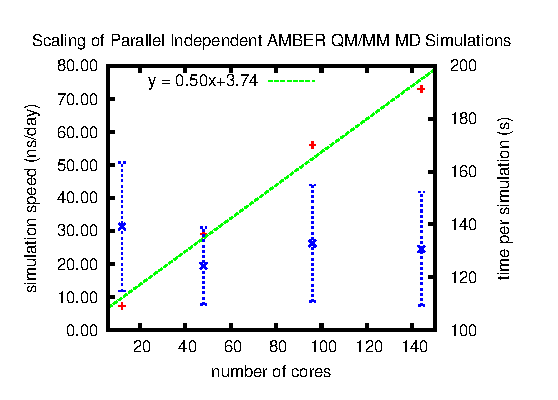
\includegraphics[width=3in]{amber_data/qmmm.eps}
\caption{
  Scaling results for ASyncRE/BigJob with the AMBER MD engine employing a
  serial quantum mechanical/molecular mechanical potential. The total number
  of cores allocated for the full REMD run was varied, while each simulation
  was run on a single core. As should be expected, performance (as measured in
  ns/day) increases linearly (green line) with the number of simulations 
  running at any given point in time. It is perhaps relevant to note that the
  performance of individual simulations is also quite consistent at different
  core counts (blue points), verifying that the linear scaling is in fact
  representative of an increase in the number of simulations running and not
  just an increased core count.
  \label{fig:amber_qmmm}  
}
\end{figure}

The efficiency of many advanced simulation models, including quantum 
mechanically based methods, is fundamentally difficult or impossible to improve 
by parallelization. However, RE-US provides a general tool for increasing the
efficiency of such simulations anyway, by increasing the statistical power of
the short trajectories that can still be obtained in a reasonable time frame.
In the present work, scaling in this way would rely exclusively on the ability 
of ASyncRE/BigJob to handle hundreds or thousands of concurrent simulations.
As a test of this (and as a basic sanity check), the performance benefit of 
increasing the pilot size was checked in conjunction with the AMBER MD engine
running a serial quantum mechanical/molecular mechanical potential with RE-US
(AMBER system 2 under Experimental Configuration). As seen in Figure 
\ref{fig:amber_qmmm} performance increases linearly with the core count and
there is no apparent cost for coordinating additional simulations. Although 
this may become an issue when individual simulation cycles become shorter
(Figure \ref{fig:amber_mm}), this is fortunately not often the case for such 
poorly (or non-) scaling simulation methods.
